\documentclass{article}

\usepackage{amsmath}
\usepackage{geometry}
\geometry{
	a4paper,
	total={170mm,257mm},
	left=20mm,
	top=20mm,
}

\usepackage{graphicx}
\usepackage{subcaption}

\begin{document}

	
For conservation laws of the form
\begin{equation}
	u_t + f(u)_x = 0, 
	\label{conservaton}
\end{equation}
or equivalently in the quasilinear form
\begin{equation}
	u_t + f'(u)u_x = 0, 
\end{equation}
we can rewrite the IIOE scheme in the following flux-differencing form
\begin{equation}
	u_i^{n} = u_i^{n - 1} - \dfrac{\tau}{h}(F_{i + 1/2} - F_{i - 1/2})
\end{equation}
if we define the average fluxes at cell interfaces depending on the sign characteristic speed $ f'(u) $(which is known from the initital state) as follows:
\[
F_{i - 1/2} = 
\begin{cases}
	\dfrac{1}{2}\left[f(u^n_{i-1}) + f(u^{n-1}_{i})\right] &  \text{if } f'(u)\big|_{\substack{x_{i-1/2}}} > 0\\
	\\
	\dfrac{1}{2}\left[f(u^{n-1}_{i-1}) + f(u^{n}_{i})\right] &  \text{if } f'(u)\big|_{\substack{x_{i-1/2}}} < 0
\end{cases}
\]


Basically when calculating the average flux at a given interface from the cell averages of the unknown function $ u(t,x) $ in neighbouring cells, we treat the upstream values implicitly and the downstream values explicitly.


\section{Examples}
\subsection{Advection with constant velocity}

\begin{equation}
	u_t + vu_x = 0, 
	\label{adv}
\end{equation}
We can write this equation as (\ref{conservaton}) with the flux function $ f(u) = vu $ with constant characteristic speed $ f'(u) = v $.

Let's assume $ v > 0 $. According to the previous section we define the average fluxes at the cell interfaces as follows:

\[
F_{i - 1/2} = \dfrac{1}{2}(vu^n_{i-1} + vu^{n-1}_{i})
\]
\[
F_{i + 1/2} = \dfrac{1}{2}(vu^n_{i} + vu^{n-1}_{i+1})
\]
The IIOE scheme becomes for $ v>0 $:
\[
u_i^{n} = u_i^{n - 1} - \dfrac{\tau}{h}\left(\dfrac{v}{2}(u^n_{i} + u^{n-1}_{i+1}) - \dfrac{v}{2}(u^n_{i-1} + u^{n-1}_{i})\right)
\]

\subsection{Burgers' equation}
\begin{equation}
	u_t + uu_x = 0, 
	\label{inviscid}
\end{equation}

We can write this equation in conservation form as (\ref{conservaton}) with the flux function $ f(u) = \dfrac{u^2}{2} $ and characteristic speed $ f'(u) = u $.

For regions, where $ f'(u) > 0 $, we define the average fluxes at the cell interfaces in a similiar manner as in the previous example:
\[
F_{i - 1/2} = \dfrac{1}{2}\left[\frac{(u^n_{i-1})^2}{2} + \frac{(u^{n-1}_{i})^2}{2} \right]
\]
\[
F_{i + 1/2} = \dfrac{1}{2}\left[\frac{(u^n_{i})^2}{2} + \frac{(u^{n-1}_{i+1})^2}{2} \right]
\]
then the scheme becomes:
\[
u_i^{n} = u_i^{n - 1} - \frac{\tau}{h}\left[
\frac{1}{2}\left(\frac{(u^n_{i})^2}{2} + \frac{(u^{n-1}_{i+1})^2}{2} \right)
 - 
\frac{1}{2}\left(\frac{(u^n_{i-1})^2}{2} + \frac{(u^{n-1}_{i})^2}{2}\right)
\right]
\]

\[
u_i^{n} = u_i^{n - 1} - \dfrac{\tau}{4h}\left[
(u^n_{i})^2 + (u^{n-1}_{i+1})^2 
- 
(u^n_{i-1})^2 - (u^{n-1}_{i})^2
\right]
\]
Putting the unknown values to the left hand side we get
\begin{equation}
u_i^{n} + \dfrac{\tau}{4h}\left[(u^n_{i})^2 - (u^n_{i-1})^2\right] = 
u_i^{n - 1} + \dfrac{\tau}{4h}\left[(u^{n-1}_{i})^2 - (u^{n-1}_{i+1})^2\right]
\label{inviscid_0}
\end{equation}


%\[
%-\dfrac{\tau}{4h}(u^n_{i-1})^2 + (1 + \dfrac{\tau}{4h}u^n_{i})u_i^{n} = 
%(1 + \dfrac{\tau}{4h}u^{n-1}_{i})u_i^{n - 1} - \dfrac{\tau}{4h}(u^{n-1}_{i+1})^2
%\]

For convinience, we show that the scheme is identical to the IIOE scheme presented in previous works, where the characteristic speeds at interfaces where defined as
\[ v^{n}_{i-1/2} = \dfrac{u^{n}_i + u^{n}_{i-1}}{2},\quad
v^{n}_{i+1/2} = \dfrac{u^{n}_i + u^{n}_{i+1}}{2} \]
Then we defined the inflow and outflow coefficients
\begin{eqnarray}
	a^{in,n}_{i-1/2} = \textrm{max}(v^{n}_{i-1/2},0),\quad 
	a^{out,n}_{i-1/2} = \textrm{min}(v^{n}_{i-1/2},0), \nonumber
	\\
	a^{in,n}_{i+1/2} = \textrm{max}(-v^{n}_{i+1/2},0),\quad 
	a^{out,n}_{i+1/2} = \textrm{min}(-v^{n}_{i+1/2},0). \nonumber
\end{eqnarray}
The diffusion term was treated with the Crank-Nicolson scheme, we ended up with the IIOE scheme for the viscous Burgers' equation
\begin{eqnarray}
	\label{viscBurg}
	u^n_i + \frac{\tau}{2h} \left(a^{in,n}_{i - 1/2} + \frac{\sigma}{h} \right) \left(u^n_i - u^n_{i-1}\right) + 
	\frac{\tau}{2h} \left(a^{in,n}_{i + 1/2} + \frac{\sigma}{h} \right) \left(u^n_i - u^n_{i+1}\right) = \\
	u^{n-1}_i - \frac{\tau}{2h} \left(\left(a^{out,n-1}_{i - 1/2} + \frac{\sigma}{h} \right) \left(u^{n-1}_i - u^{n-1}_{i-1}\right) + 
	\left(a^{out,n-1}_{i + 1/2} + \frac{\sigma}{h} \right) \left(u^{n-1}_i - u^{n-1}_{i+1}\right)\right).\nonumber
\end{eqnarray}
Assuming $ u > 0 $ we get \\
\[
a^{in,n}_{i-1/2} = \dfrac{u^{n}_i + u^{n}_{i-1}}{2},\quad a^{out,n}_{i-1/2} = 0,\quad a^{in,n}_{i + 1/2} = 0,\quad a^{out,n}_{i+1/2} = -\dfrac{u^{n}_i + u^{n}_{i+1}}{2}.
\]
Substituting into the numerical scheme and assuming $ \sigma = 0 $ we end up with
\begin{equation}
	u^n_i + \frac{\tau}{2h} \dfrac{u^{n}_i + u^{n}_{i-1}}{2} \left(u^n_i - u^n_{i-1}\right)
	= 
	u^{n-1}_i - \frac{\tau}{2h} 
	\left(-\dfrac{u^{n}_i + u^{n}_{i+1}}{2}\right) \left(u^{n-1}_i - u^{n-1}_{i+1}\right)
\end{equation}
after simplifying we get
\begin{equation}
	\label{inviscid_1}
u_i^{n} + \dfrac{\tau}{4h}\left[(u^n_{i})^2 - (u^n_{i-1})^2\right] = 
u_i^{n - 1} + \dfrac{\tau}{4h}\left[(u^{n-1}_{i})^2 - (u^{n-1}_{i+1})^2\right]
\end{equation}
which coincides with (\ref{inviscid_0}) derived previously.

\subsection{Traffic flow}
For the LWR model with flux $ f(\rho) = \rho (1 - \rho) $ and characteristic speed $ f'(\rho) = 1 - 2\rho $ we get
\[
F_{i - 1/2} = \frac{1}{2}\left[\rho^n_{i-1} (1 - \rho^n_{i-1}) + \rho^{n-1}_{i} (1 - \rho^{n-1}_{i}) \right]
\]
\[
F_{i + 1/2} = \frac{1}{2}\left[\rho^n_{i} (1 - \rho^n_{i}) + \rho^{n-1}_{i+1} (1 - \rho^{n-1}_{i+1}) \right]
\]
then the scheme becomes
\[
	\rho_i^{n} = \rho_i^{n - 1} - \dfrac{\tau}{h}
	\left(\frac{1}{2}\left[\rho^n_{i} (1 - \rho^n_{i}) + \rho^{n-1}_{i+1} (1 - \rho^{n-1}_{i+1}) \right]
	 - 
	 \frac{1}{2}\left[\rho^n_{i-1} (1 - \rho^n_{i-1}) + \rho^{n-1}_{i} (1 - \rho^{n-1}_{i}) \right]\right)
\]

\[
\rho_i^{n} + \frac{\tau}{2h}\left[\rho^n_{i} (1 - \rho^n_{i}) - \rho^n_{i-1} (1 - \rho^n_{i-1})\right]
=
\rho_i^{n - 1} - \dfrac{\tau}{2h}\left[\rho^{n-1}_{i+1} (1 - \rho^{n-1}_{i+1}) - \rho^{n-1}_{i} (1 - \rho^{n-1}_{i})\right]
\]
Now let us compare the result with our previously derived IIOE scheme.\\
Assuming $ f'(\rho) = 1 - 2\rho > 0 $ we get \\
\[
a^{in,n}_{i-1/2} = 1 - (\rho^n_{i-1} + \rho^n_{i}),\quad a^{out,n}_{i-1/2} = 0,\quad a^{in,n}_{i + 1/2} = 0 \text{ and } a^{out,n}_{i+1/2} = -\left(1 - (\rho^n_{i} + \rho^n_{i+1}) \right)
\]
Substituting into the numerical scheme and assuming we end up with
\[
	\rho^n_i + \frac{\tau}{2h} \left[1 - (\rho^n_{i-1} + \rho^n_{i})\right] \left(\rho^n_i - \rho^n_{i-1}\right)
	= 
	\rho^{n-1}_i - \frac{\tau}{2h} 
	\left[-\left(1 - (\rho^{n-1}_{i} + \rho^{n-1}_{i+1}) \right)\right] \left(\rho^{n-1}_i - \rho^{n-1}_{i+1}\right)
\]

\[
\rho^n_i + \frac{\tau}{2h} \left[\left(\rho^n_i - \rho^n_{i-1}\right) - ((\rho^n_{i})^2 - (\rho^n_{i-1})^2)\right] 
= 
\rho^{n-1}_i + \frac{\tau}{2h} \left[\left(\rho^{n-1}_i - \rho^{n-1}_{i+1}\right) - ((\rho^{n-1}_{i})^2 - (\rho^{n-1}_{i+1})^2)\right] 
\]
which is the same that we got earlier.
\subsection{Advection with variable velocity}
\begin{equation}
	u_t + vu_x = 0, 
	\label{color}
\end{equation}
where $ v = v(x) $. We rewrite (\ref{color}) in the equivalent form

\begin{equation}
	u_t + (vu)_x - uv_x = 0,
\end{equation}
where one can recognize a conservation term and a source term. The IIOE can be equivalently written in terms of fluxes, if we define the numerical fluxes approprietly.

For this problem with a variable velocity, the flux is not only a function of $ u(t,x) $, it depends also on the position $ x $ explicitly. We define the flux as
\[
f(x, u(t, x)) = v(x) u(t, x),
\]
where the characteristic speed $ v(x) $ is a known function. According to previous derivations, we should calculate the numerical flux at a given interface as
\[
F_{i - 1/2} = 
\begin{cases}
	\dfrac{1}{2}(v_{i-1}u^n_{i-1} + v_{i}u^{n-1}_{i}) &  \text{if } v_{i-1/2} > 0\\
	\\
	\dfrac{1}{2}(v_{i-1}u^{n-1}_{i-1} + v_{i}u^{n}_{i}) &  \text{if } v_{i-1/2} < 0.
\end{cases}
\]
To discretize the source term, we assume, that it depends on the cell average in space and it is averaged in time also value over a time step $ \tau $.
\begin{equation}
	-uv_x \approx -\frac{1}{2}(u_i^n + u_i^{n-1})\frac{v_{i+1/2} - v_{i-1/2}}{h}.
\end{equation}
This way we get a slightly different scheme as before.

However, it is reasonable to assign the exact speed to the corresponding interface, and we need a reconstruction only for the unknown function $ u(t,x) $. We can define a numerical flux function depending on the sign characteristic speed $ v(x) $ as follows:
\[
F_{i - 1/2} = 
\begin{cases}
	\dfrac{v_{i-1/2}}{2}(u^n_{i-1} + u^{n-1}_{i}) &  \text{if } v_{i-1/2} > 0\\
	\\
	\dfrac{v_{i-1/2}}{2}(u^{n-1}_{i-1} + u^{n}_{i}) &  \text{if } v_{i-1/2} < 0.
\end{cases}
\]
Substituting the flux calculated that way the scheme agrees with the IIOE scheme presented in previous works.

\section{Limited scheme}
Higher order schemes suffer from numerical dispersion. Unphysical oscillations can occur near sharp changes of the solution. A remedy to this is to use limiters.

As discussed in the previous section, we can define the avarege flux as
\[
F_{i - 1/2} = 
\begin{cases}
	\dfrac{1}{2}\left[f(u^n_{i-1}) + f(u^{n-1}_{i})\right] &  \text{if } f'(u)\big|_{\substack{x_{i-1/2}}} > 0\\
	\\
	\dfrac{1}{2}\left[f(u^{n-1}_{i-1}) + f(u^{n}_{i})\right] &  \text{if } f'(u)\big|_{\substack{x_{i-1/2}}} < 0
\end{cases}
\]
where we are avareging the fluxes calculated implicitly from upstream values and explicitly from downstream values. This suggests that we should calculate a weighted average instead as a possible improvement:

\[
F_{i - 1/2}^{\theta} = 
\begin{cases}
	(1-\theta_{i-1/2})f(u^n_{i-1}) + \theta_{i-1/2} f(u^{n-1}_{i}) &  \text{if } f'(u)\big|_{\substack{x_{i-1/2}}} > 0\\
	\\
	\theta_{i-1/2} f(u^{n-1}_{i-1}) + (1-\theta_{i-1/2}) f(u^{n}_{i}) &  \text{if } f'(u)\big|_{\substack{x_{i-1/2}}} < 0
\end{cases}
\]
It might be illuminating to write the flux as:
\[
F_{i - 1/2}^{\theta} = 
\begin{cases}
	f(u^n_{i-1}) - \theta_{i-1/2} \left[f(u^n_{i-1}) - f(u^{n-1}_{i})\right] &  \text{if } f'(u)\big|_{\substack{x_{i-1/2}}} > 0\\
	\\
	f(u^{n}_{i}) - \theta_{i-1/2} \left[f(u^{n}_{i}) - f(u^{n-1}_{i-1})\right] &  \text{if } f'(u)\big|_{\substack{x_{i-1/2}}} < 0
\end{cases}
\]
For $ \theta_{i-1/2} = \frac{1}{2} $ we get the basic scheme, for $ \theta_{i-1/2} = 0 $ we get the implicit upwind scheme.

It is challenging to define the weighting coefficient $ \theta_{i-1/2} $ properly. Since we know that solutions of conservation laws don't generate new extrema as time evolves, one possible way is to limit the flux based on a "min, max" restriction of the numerical solution by defining for every cell $ u_i^{min} $, $ u_i^{max} $ in an appropiate way using known values.

\subsection{Advection with constant velocity}
Here we take advantage of the fact, that the characteristic speed doesn't change sign. With given inflow boundary condition at every time step, we can calculate cell avareges one by one directly in the direction of wave propagation. Based on that fact we can bound the cell averages between $ u_i^{min} $, $ u_i^{max} $.
For advection with $ v = 1 $ the limited scheme becomes:
\[
u_i^{n} = u_i^{n - 1} - 
\frac{\tau}{h}
\left[
\left((1 - \theta_{i+1/2})u^n_{i} + \theta_{i+1/2}u^{n-1}_{i+1}\right) - \left((1 - \theta_{i-1/2})u^n_{i-1} + \theta_{i-1/2}u^{n-1}_{i}\right)
\right]
\]
\[
u_i^{n} + \frac{\tau}{h}(1 - \theta_{i+1/2})u^n_{i} - \frac{\tau}{h}(1 - \theta_{i-1/2})u^n_{i-1} = 
u_i^{n - 1} - 
\frac{\tau}{h}
\left(
 \theta_{i+1/2}u^{n-1}_{i+1} - \theta_{i-1/2}u^{n-1}_{i}
\right)
\]
Expressing $ u^n_{i} $ we get
\begin{equation}
u_i^n = \frac{u_i^{n - 1} + 
	\dfrac{\tau}{h}
	\left[
	(1 - \theta_{i-1/2})u^n_{i-1} - \theta_{i-1/2}u^{n-1}_{i}
	\right]}{1+\dfrac{\tau}{h}(1 - \theta_{i+1/2})}
\end{equation}
We want
\[
u_i^{min} \leq u^n_i \leq u_i^{max} 
\]
substituting we get
\begin{equation}
u_i^{min} \leq
 \frac{u_i^{n - 1} + 
 	\dfrac{\tau}{h}
 	\left[
 	(1 - \theta_{i-1/2})u^n_{i-1} - \theta_{i-1/2}u^{n-1}_{i}
 	\right]}{1+\dfrac{\tau}{h}(1 - \theta_{i+1/2})}
\leq u_i^{max}
\label{minmax}
\end{equation}
For $ v > 0 $, we start at the left boundary with $ \theta_{1 / 2} = 1/2 $ and the wieghts at interfaces inside the domain calculate in order to satisfy \eqref{minmax}.

Let us compare 2 different profiles on a coarse grid. In case of a discontinous rectangular wave, it works fine - the exact solution would have either the global maximum or global minimum calculated from the initial state.
In the case of a continous hump, on coarser grids this approach tends to sharpen the solution on the left side and smears on the right side, as it is documented in the figures. Min, max values are set to global extremes.

\begin{figure}[h!]
	\begin{subfigure}{.5\textwidth}
	\centering
	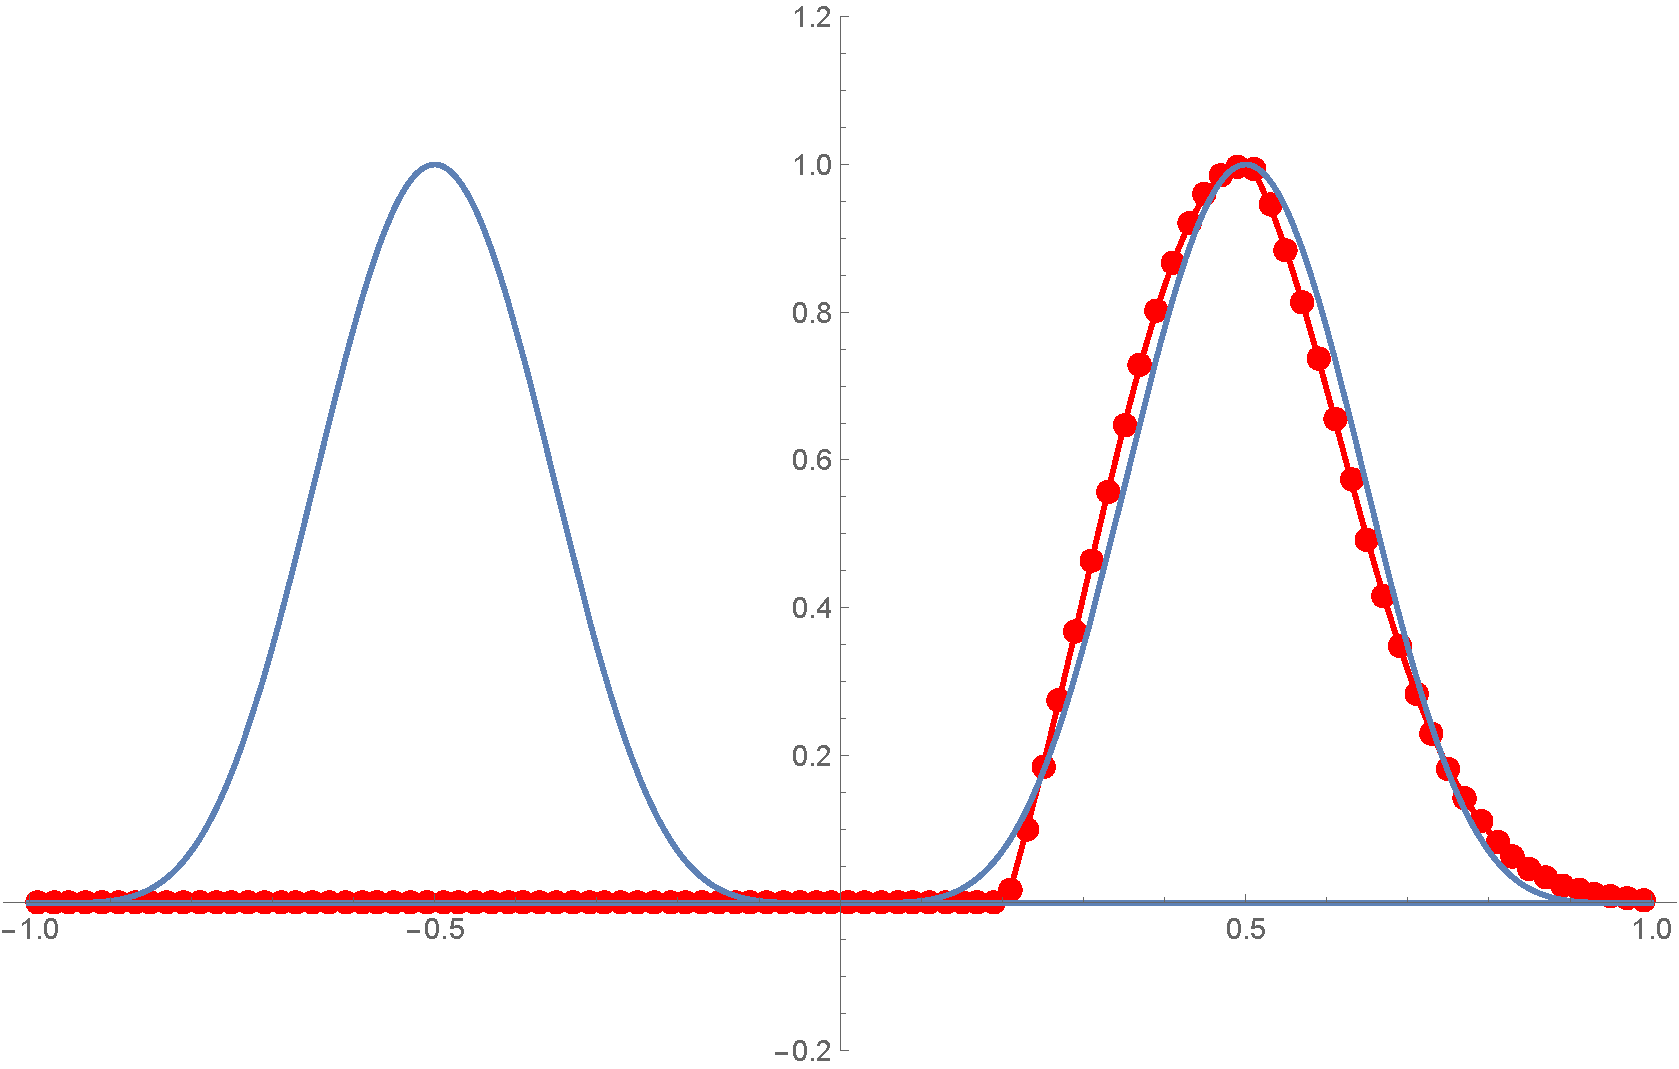
\includegraphics[width=\textwidth]{smoothHump}
	\end{subfigure}
	\begin{subfigure}{.5\textwidth}
		\centering
		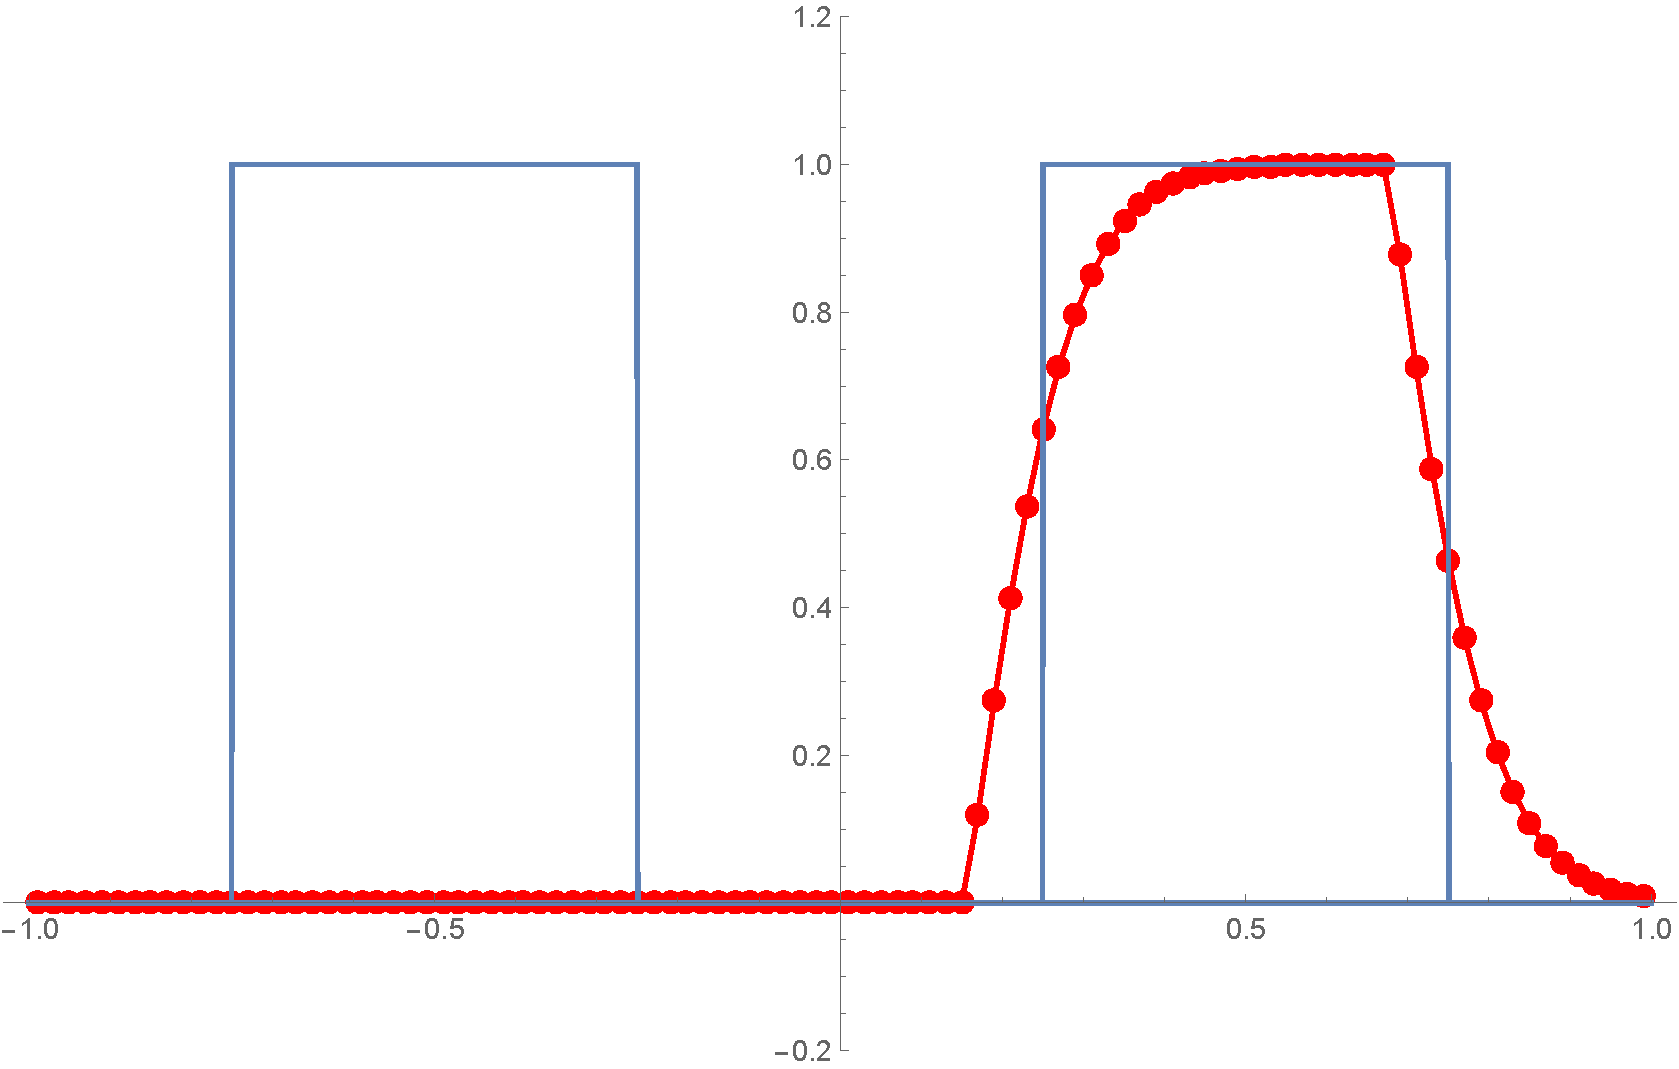
\includegraphics[width=\textwidth]{constant_discontinous}
	\end{subfigure}
\end{figure}

\subsection{Burgers' equation}

Here again, we start with the assumption that the cell averages can be calculated from upstream values at every time step(starting at boundary or where the solution is stationary).

For regions, where the characteristic speed $ f'(u) > 0 $ the limited scheme is

\begin{equation}
	u_i^{n} = u_i^{n - 1} - \frac{\tau}{h}\left[
	\left((1 - \theta_{i+1/2})\frac{(u^n_{i})^2}{2} + \theta_{i+1/2}\frac{(u^{n-1}_{i+1})^2}{2} \right)
	- 
	\left((1 - \theta_{i-1/2})\frac{(u^n_{i-1})^2}{2} + \theta_{i-1/2}\frac{(u^{n-1}_{i})^2}{2}\right)
	\right]
\end{equation}
Assuming the only unknown is $ u_i^n $ we put on the left hand side to get
\[
u_i^{n} + \frac{\tau}{h}(1 - \theta_{i+1/2})\frac{(u^n_{i})^2}{2}
=
u_i^{n - 1} - \frac{\tau}{h}\left[
\theta_{i+1/2}\frac{(u^{n-1}_{i+1})^2}{2}
- 
\left((1 - \theta_{i-1/2})\frac{(u^n_{i-1})^2}{2} + \theta_{i-1/2}\frac{(u^{n-1}_{i})^2}{2}\right)
\right]
\]
which is a quadratic equation.\\
We describe a possible way to calculate the cell averages.
It might not be practical to solve the quadratic equation directly(maybe we could use Newton's method). We can write the equation as
\[
u_i^{n}\left(1 + \frac{\tau}{h}(1 - \theta_{i+1/2})\frac{u^n_{i}}{2}\right)
=
u_i^{n - 1} - \frac{\tau}{h}\left[
\theta_{i+1/2}\frac{(u^{n-1}_{i+1})^2}{2}
- 
\left((1 - \theta_{i-1/2})\frac{(u^n_{i-1})^2}{2} + \theta_{i-1/2}\frac{(u^{n-1}_{i})^2}{2}\right)
\right]
\]
where the coefficient for $ u^n_i $ depends on the unknown.
We want to ensure that our numerical solution doesn't create new extrema. 
\[
u_i^{min} \leq u^n_i \leq u_i^{max} 
\]

\begin{equation}
	u_i^{min} \leq 
	\frac{u_i^{n - 1} - \dfrac{\tau}{2h}\left[
		\theta_{i+1/2}(u^{n-1}_{i+1})^2
		- 
		\left((1 - \theta_{i-1/2})(u^n_{i-1})^2 + \theta_{i-1/2}(u^{n-1}_{i})^2\right)
		\right]}{1 + \dfrac{\tau}{2h}(1 - \theta_{i+1/2})u^n_{i}}
	\leq u_i^{max} 
	\label{Burgminmax}
\end{equation}

We describe below one possibility. We calculate $ u^n_i $ iteratively:
\begin{itemize}
	\item First we calculate 
	\[
	u_i^{n,1} =
	\frac{u_i^{n - 1} - \dfrac{\tau}{2h}\left[
		\theta_{i+1/2}(u^{n-1}_{i+1})^2
		- 
		\left((1 - \theta_{i-1/2})(u^n_{i-1})^2 + \theta_{i-1/2}(u^{n-1}_{i})^2\right)
		\right]}{1 + \dfrac{\tau}{2h}(1 - \theta_{i+1/2})u_i^{*}},
	\]
	with the basic scheme, where $ u_i^{*} $ is a guess value for $ u_i^{n}$, the weights are set to 1/2.
	\item if $u_i^{min} \leq  u_i^{n,1} \leq u_i^{max} $ we redefine the weigths to satisfy
	\[
	u_i^{min} \leq 
	\frac{u_i^{n - 1} - \dfrac{\tau}{2h}\left[
		\theta_{i+1/2}(u^{n-1}_{i+1})^2
		- 
		\left((1 - \theta_{i-1/2})(u^n_{i-1})^2 + \theta_{i-1/2}(u^{n-1}_{i})^2\right)
		\right]}{1 + \dfrac{\tau}{2h}(1 - \theta_{i+1/2})u_i^*}
	\leq u_i^{max} 
	\]
	\item iterate as long as the residual doesn't drop below the desired value(we calculate the weights in the first iteration only)
\end{itemize}

\begin{figure}[h!]
	\begin{subfigure}{.5\textwidth}
		\centering
		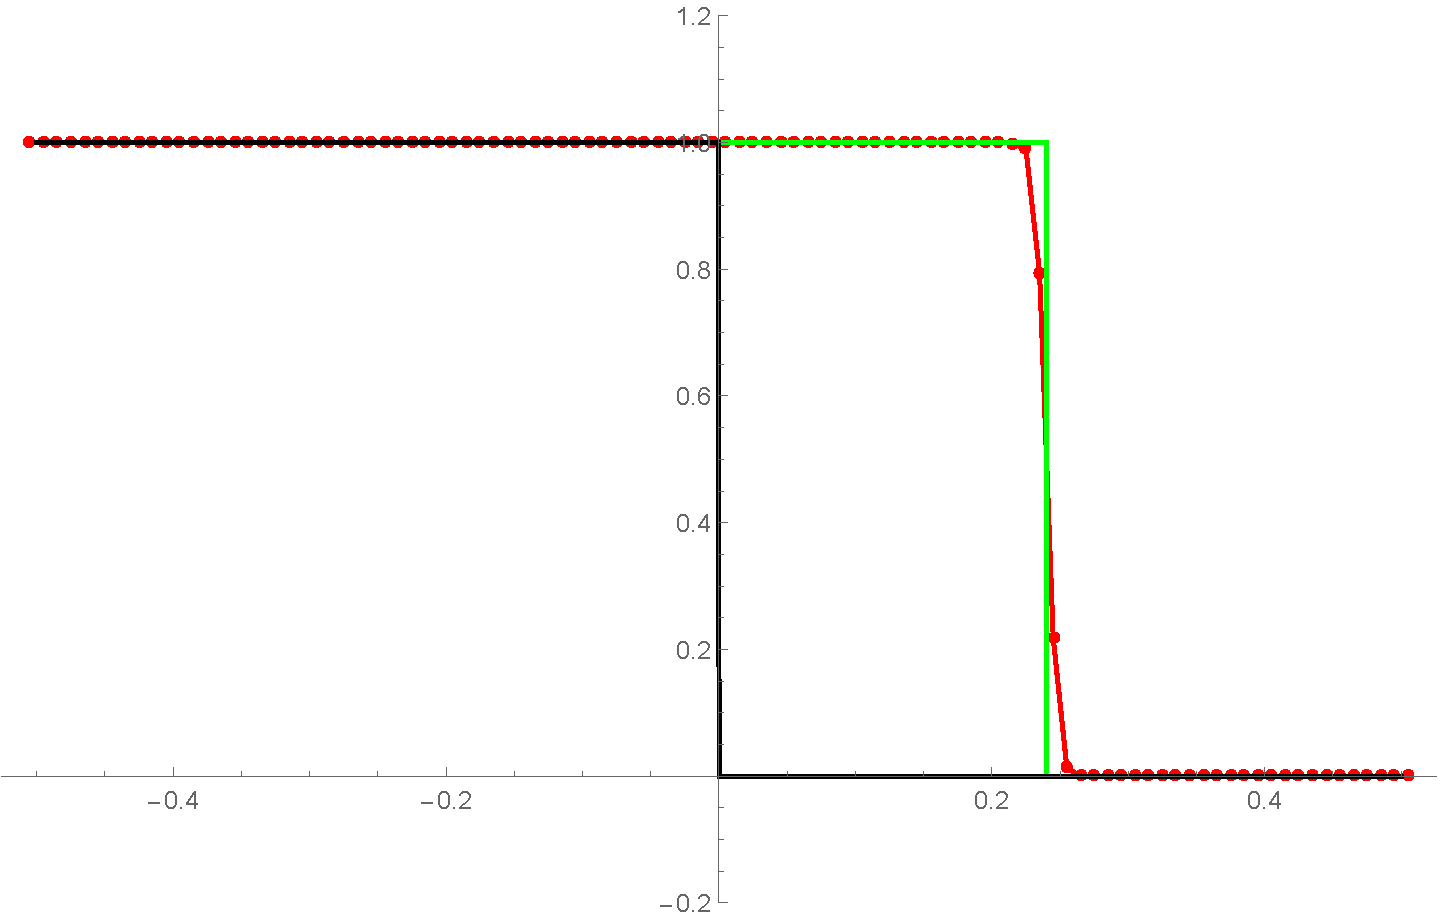
\includegraphics[width=\textwidth]{travel}
		\caption{$ n = 100 $, $ \tau = h $, min, max is set to global extrema}
	\end{subfigure}
	\begin{subfigure}{.5\textwidth}
		\centering
		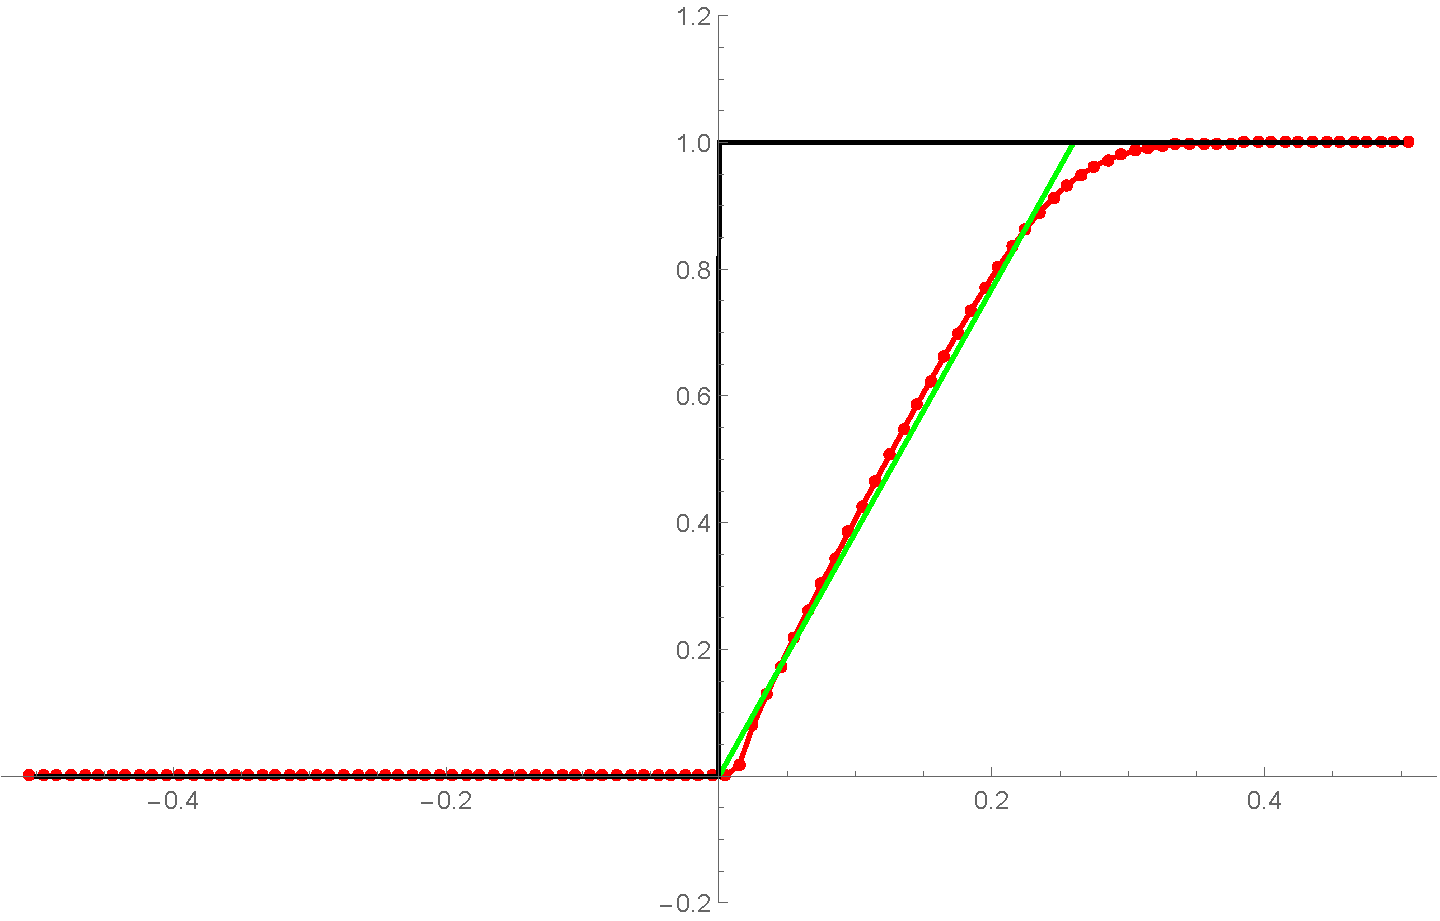
\includegraphics[width=\textwidth]{rare}
	\end{subfigure}
\end{figure}

\begin{figure}[h!]
	\begin{subfigure}{.5\textwidth}
		\centering
		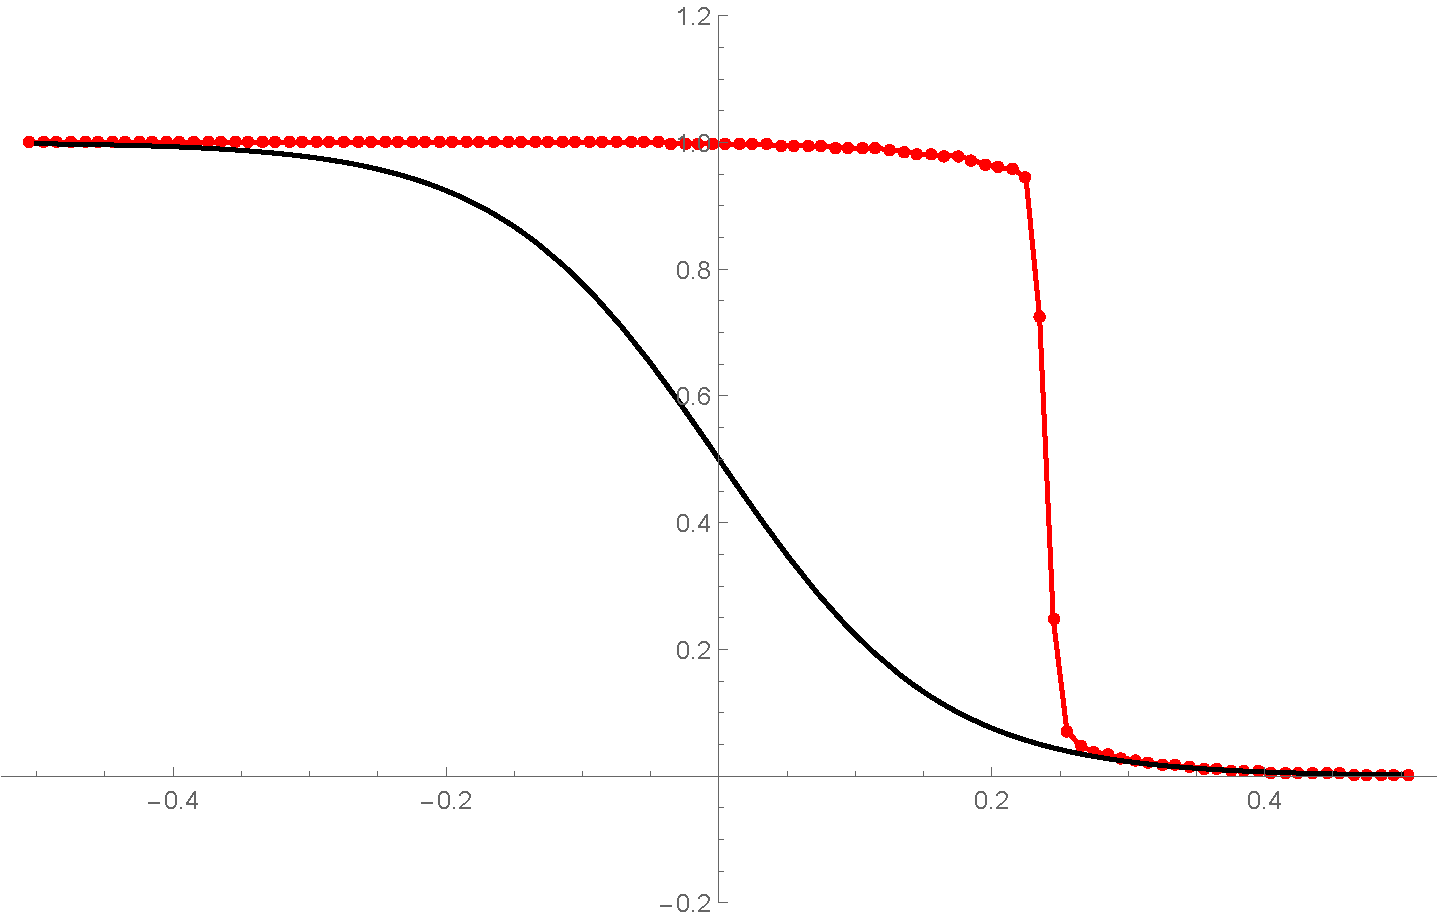
\includegraphics[width=\textwidth]{shock}
		\caption{$ n = 100 $, $ \tau = h $, min, max calculated from upstream values at the previous time step}
	\end{subfigure}
	\begin{subfigure}{.5\textwidth}
		\centering
		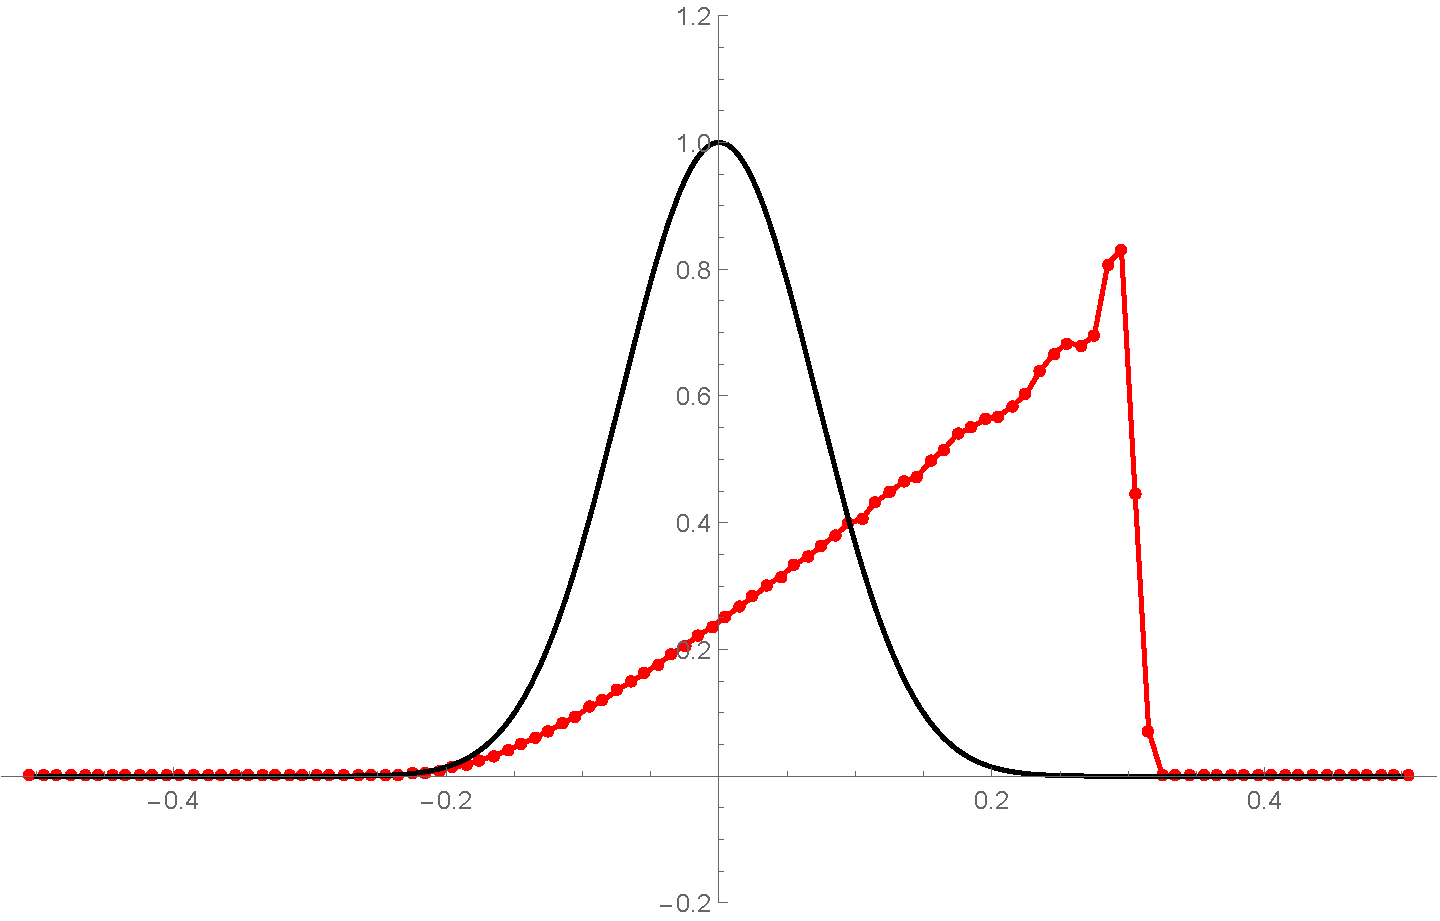
\includegraphics[width=\textwidth]{triang}
	\end{subfigure}
\end{figure}

\[
F_{i-1/2} = s_{i-1/2}^{in, k} \, \dfrac{1}{2}\left(f^{n,k}_{i-1} + f^{n-1}_{i}\right) + s_{i-1/2}^{out} \, \dfrac{1}{2}\left(f^{n-1}_{i-1} + f^{n,k}_{i}\right)
\]
\[
s_{i-1/2}^{in, k} = \max\left(\frac{f'(u_{i-1}^{n,k}) + f'(u_{i}^{n,k})}{2}, 0\right), \quad s_{i-1/2}^{out} = \frac{f'(u_{i-1}^{n-1}) + f'(u_{i}^{n-1})}{2}
\]

\end{document}